\documentclass[11pt,a4paper]{article}

\usepackage[margin=1in]{geometry}
\usepackage{amsmath,amssymb}
\usepackage{fontspec}
% Times New Roman (Nimbus Roman metric-compatible OpenType typeface)
\setmainfont{Nimbus Roman}
\usepackage{graphicx}
\usepackage{booktabs}
\usepackage{hyperref}

\hypersetup{
    colorlinks=true,
    linkcolor=blue,
    citecolor=blue,
    urlcolor=blue
}

\title{\textbf{Coupling Crustal Geodesy, 3D Seismicity, and Nonlinear Waveform Lyapunov Dynamics for Pre-, Co-, and Post-Seismic Fault Kinematics: Application to the 2011 Van (\textit{M}\textsubscript{w} 7.1) and 2023 Kahramanmara\c{s} (\textit{M}\textsubscript{w} 7.8) Earthquakes}}

\author{\textbf{Oguz Bolat}\\
Department of Geomatics Engineering, Y{\i}ld{\i}z Technical University\\
Istanbul, Turkey\\
\texttt{hoguzbolat@gmail.com}}
\date{\today}

\begin{document}

\maketitle

\begin{abstract}
Constraining fault geometry, pre-seismic strain accumulation, dynamic coseismic slip, and post-seismic state evolution requires synthesizing geodetic deformation fields, seismicity distributions, and seismic waveform dynamics. Traditional methodologies evaluate these data streams in isolation: geodetic inversions estimate static dislocation geometry and slip amplitude; hypocentre clustering maps aftershock clouds; and waveform analyses characterize source rupture properties. Here, we present \texttt{chaosmap}, an end-to-end high-performance C++23 pipeline that couples continuous GNSS geodesy, 3D hypocentre principal component regression, and two complementary Lyapunov formulations: (1) Geodetic Finite-Time Lyapunov Exponents ($L_{\text{geo}}$), which detect Lagrangian coherent strain structures and deformation barriers via particle advection in the continuous velocity gradient tensor; and (2) Broadband Seismic Waveform Lyapunov Analysis ($L_{\text{seis}}$), which quantifies temporal predictability loss and phase-space divergence via Wolf and Rosenstein largest Lyapunov exponent algorithms on ambient crustal noise after Lee (1972) coda duration exclusion and ocean microseism control-band differencing.

We validate the analytical elastic dislocation kernel against the Okada (1985) check values, which it reproduces to within their four-significant-figure rounding (absolute error $<5\times 10^{-6}\text{ m}$ for unit slip), and test the complete pipeline on two major tectonic events in Turkey: the 2011 Van-Erci\c{s} ($M_w\,7.1$) blind reverse earthquake and the 2023 Kahramanmara\c{s} ($M_w\,7.8$) East Anatolian strike-slip rupture. In the 2011 Van event, multi-station GNSS trajectory inversion yields a fault striking $248.0^\circ$, dipping $50.5^\circ$, with a geodetic moment of $5.30\times 10^{19}\text{ N}\cdot\text{m}$ ($M_w\,7.08$) and peak slip of $2.48\text{ m}$, achieving a variance reduction of $97.39\%$. $L_{\text{seis}}$ exhibits a pre-event 3-day array-anomaly ROC AUC of $0.867$, which is not significant ($p = 0.125$, the smallest $p$-value a circular time-slide null can return with eight pre-event days), and post-minus-pre Wolf exponent drops that decrease in magnitude with epicentral distance at the three stations that returned data ($\Delta \lambda_1 = -0.57\text{ bits/s}$ at TVAN, $23.7\text{ km}$; $-0.33$ at GEVA, $60.0\text{ km}$; $-0.07$ at DYDN, $92.8\text{ km}$). In the 2023 Kahramanmara\c{s} rupture, station EKZ1 records a horizontal coseismic displacement of $4.67\text{ m}$, and distributed slip inversion yields a peak slip of $22.05\text{ m}$ (top-quartile mean $11.99\text{ m}$), geodetic $M_w\,7.78$, and variance reduction of $77.47\%$. Because daily GNSS solutions combine the $M_w\,7.8$ mainshock with the $M_w\,7.5$ Elbistan event of the same day, this single-plane model is only an approximation, and its peak-slip patch, adjacent to EKZ1 and the $M_w\,7.5$ rupture, is an artefact of the parameterisation. Four-panel kinematic synthesis maps (Before, Moved, After, and Change) provide a unified framework for resolving crustal stress accumulation and rupture boundaries.
\end{abstract}

\section{Introduction}
Quantifying the kinematic behaviour of seismogenic fault systems across their full earthquake cycle remains a central challenge in geophysical continuum mechanics. Understanding how a fault transforms from a locked pre-seismic state to high-velocity slip, and subsequently to a distributed post-seismic relaxation zone, requires mapping:
\begin{enumerate}
    \item \textbf{Before the earthquake:} Background inter-seismic strain rates, regional micro-seismicity alignments, and crustal phase-space stability.
    \item \textbf{During the earthquake (``How much it moved''):} Coseismic surface displacement vectors, 3D fault geometry (strike, dip, rake, depth), and heterogeneous distributed slip amplitude on fault patches.
    \item \textbf{After the earthquake:} Post-seismic aftershock rupture clouds, secondary fault splays, and post-rupture stress redistributions.
    \item \textbf{Before-vs-After change:} Differential state shifts, strike rotations, fault centroid migrations, and dynamic phase-space anomalies.
\end{enumerate}

To date, mathematical frameworks for fault analysis have bifurcated. On the one hand, geodetic geodesy relies on static elastic half-space dislocations \cite{okada1985} driven by Global Navigation Satellite System (GNSS) observations to infer slip distributions. On the other hand, non-linear time series analysis has applied chaos theory and dynamical systems techniques (e.g., Lyapunov exponents, sample entropy, fractal correlation dimension) to seismic time series, searching for non-linear precursors or localized changes in ambient crustal predictability \cite{wolf1985, rosenstein1993, sarwar2023}. However, these approaches have rarely been integrated into an automated, quantitative spatial framework.

Turkey occupies an active tectonic wedge squeezed westward between the colliding Arabian and Eurasian plates. The motion is accommodated primarily by the dextral North Anatolian Fault Zone (NAFZ), the sinistral East Anatolian Fault Zone (EAFZ), and the complex collision/thrust structures of the Bitlis-Zagros suture zone in Eastern Anatolia. To study this spectrum of deformation, we investigate two landmark earthquakes representing contrasting tectonic environments:
\begin{itemize}
    \item \textbf{The 23 October 2011 Van-Erci\c{s} Earthquake ($M_w\,7.1$):} A blind reverse rupture north of Lake Van with minimal primary surface rupture, requiring geodetic inversion and 3D aftershock geometry to delineate fault parameters. Four continuous broadband seismic stations (`DYDN`, `GEVA`, `TVAN`, `VMUR`) operated within $100\text{ km}$ of the epicenter.
    \item \textbf{The 6 February 2023 Kahramanmara\c{s} Mainshock ($M_w\,7.8$):} A major strike-slip rupture on the East Anatolian Fault Zone with left-lateral surface offsets exceeding $6\text{ m}$ and exceptional near-field GNSS coseismic displacements (up to $4.67\text{ m}$ horizontally at station EKZ1).
\end{itemize}

In this work, we present \texttt{chaosmap}, an open-source, reproducible C++23 computational architecture that synthesizes continuous GNSS geodesy, 3D hypocentre manifolds, and two competing implementations of non-linear Lyapunov exponents ($L_{\text{geo}}$ and $L_{\text{seis}}$) into publication-quality four-panel kinematic synthesis cartography.

\section{Materials and Methods}

\subsection{Data Sources and Observational Materials}
The \texttt{chaosmap} pipeline unifies three independent geophysical observational data streams:
\begin{enumerate}
    \item \textbf{Continuous GNSS Time-Series:} Daily position coordinates in the IGS20 reference frame are retrieved from the Nevada Geodetic Laboratory (NGL) archive, encompassing 273 permanent GNSS stations across Turkey. Station trajectory histories span from 2005 through 2024, providing multi-year inter-seismic velocity baselines and high-precision daily coordinates before and after major events. Documented instrumental offsets, antenna replacements, and known earthquake offsets are cross-referenced with the NGL `steps.txt` metadata catalog.
    \item \textbf{Regional Seismicity Catalog:} Earthquake hypocentral locations, origin times, focal depths, and magnitudes are extracted from the official Disaster and Emergency Management Authority (AFAD) earthquake catalog. Events with $M \ge 2.5$ inside the rectangular study region of each case are partitioned into a 5-year pre-seismic background window ($t_{\text{event}} - 5\text{ yr} \le t < t_{\text{event}}$) and a 120-day post-seismic aftershock catalog ($t_{\text{event}} \le t \le t_{\text{event}} + 120\text{ d}$).
    \item \textbf{Broadband Continuous Seismic Waveforms:} Raw 3-component continuous waveform archives (vertical and horizontal channels sampled at 50 Hz) are ingested directly from the Turkish National Seismic Network (TDVMS) repository in miniSEED-2 binary format wrapped in ZIP archives.
\end{enumerate}

\subsection{GNSS Trajectory Decomposition and Coseismic Step Estimation}
For each station, the horizontal position vector $\mathbf{x}(t) = [e(t), n(t)]^T$ is modelled over an inter-seismic baseline $t \in [t_{\text{event}} - T_{\text{pre}}, t_{\text{event}}]$ using robust non-parametric paired slopes (MIDAS) \cite{blewitt2016}. Each daily solution $t_i$ is paired with the first solution $t_j$ at least one year later, provided $t_j - t_i \le 1\text{ yr} + 15\text{ d}$ and no documented step falls in $(t_i, t_j]$:
\begin{equation}
\mathbf{v} = \text{median}\left\{ \frac{\mathbf{x}(t_j) - \mathbf{x}(t_i)}{t_j - t_i} \right\}
\end{equation}
with a second median after trimming slopes more than $2\sigma$ (MAD-based) from the first. Because the pairs are separated by one year, annual hydrological and thermal cycles cancel without parametric fitting.

The coseismic displacement vector $\Delta \mathbf{u} = [\Delta e, \Delta n, \Delta u]^T$ is extracted from detrended daily positions before and after the event day $t_0$ (the daily solution of the event day itself is excluded):
\begin{equation}
\Delta \mathbf{u} = \text{median}_{t \in [t_0 + 1\text{ d},\, t_0 + 16\text{ d}]} (\mathbf{x}(t) - \mathbf{v}t) - \text{median}_{t \in [t_0 - 21\text{ d},\, t_0 - 1\text{ d}]} (\mathbf{x}(t) - \mathbf{v}t)
\end{equation}
The post-event window therefore also contains up to 16 days of early postseismic motion.
In parallel, a full trajectory model incorporating Heaviside step functions for documented equipment changes (from the NGL `steps.txt` database), coseismic offsets, and post-seismic logarithmic relaxation $\ln(1 + \Delta t / \tau)$ is inverted via Singular Value Decomposition (SVD) with covariance propagation.

\subsection{Elastic Dislocation Modeling and Distributed Slip Inversion}
Surface displacements due to slip on a rectangular dislocation embedded in an isotropic, homogeneous elastic half-space are calculated using the exact closed-form expressions of Okada (1985) \cite{okada1985}. A fault patch $\mathcal{P}_k$ is parameterized by centroid position $(x_k, y_k, d_k)$, along-strike length $L_k$, down-dip width $W_k$, strike azimuth $\phi$, dip angle $\delta$, and slip vector $\mathbf{s}_k = [s_{\text{strike}}, s_{\text{dip}}]^T$.

The Green's function matrix $\mathbf{G} \in \mathbb{R}^{3M \times 2K}$ relates the slip vector $\mathbf{s} \in \mathbb{R}^{2K}$ across all $K$ patches to the predicted coseismic displacements at $M$ GNSS stations:
\begin{equation}
\mathbf{d} = \mathbf{G}\mathbf{s} + \mathbf{e}, \quad \mathbf{e} \sim \mathcal{N}(\mathbf{0}, \Sigma_{\mathbf{d}})
\end{equation}
where $\Sigma_{\mathbf{d}}$ is the data covariance matrix composed of observational standard deviations.

The inversion proceeds in two stages. First, a single rectangular plane is fitted: its initial length and width follow the Wells and Coppersmith (1994) \cite{wells1994} scaling for the catalog magnitude, and a grid search over centroid offsets ($\pm 18\text{ km}$), strike ($\pm 16^\circ$), dip ($\pm 10^\circ$), and length ($0.8$--$1.25\times$) around the event prior (1125 candidates), followed by a coordinate pattern search, minimises the weighted misfit of a two-component (strike-, dip-slip) least-squares fit with weak damping towards the catalog rake and moment. Vertical components are down-weighted by a factor of 2 relative to their formal uncertainties throughout.

Second, the best plane is divided into $8 \times 4$ (strike $\times$ dip) patches. To recover continuous slip variations while avoiding non-physical oscillatory slip distributions, we solve the regularized weighted least-squares problem:
\begin{equation}
\min_{\mathbf{s}} \left\{ \| \Sigma_{\mathbf{d}}^{-1/2} (\mathbf{d} - \mathbf{G}\mathbf{s}) \|_2^2 + \gamma^2 \| \mathbf{L}\mathbf{s} \|_2^2 + \beta^2 \| \mathbf{s} - \mathbf{s}_{\text{ref}} \|_2^2 \right\}
\end{equation}
where $\mathbf{L}$ is the discrete 2D finite-difference Laplacian between adjacent strike and dip patches (with a small diagonal damping), $\gamma = \max\!\left(0.5,\ 0.35\,\|\Sigma_{\mathbf{d}}^{-1/2}\mathbf{G}\|_F / \sqrt{2K}\right)$ scales the smoothing to the data kernel, and $\mathbf{s}_{\text{ref}}$ is the single-plane slip tapered by $1.25 \sin(\pi\,\xi)\sin(\pi\,\zeta)$ in normalised along-strike and down-dip patch position, with $\beta = 0.45\gamma$ (doubled on the dip-slip component for strike-slip events, which pulls dip slip towards half its reference value). The problem is solved by SVD least squares without sign constraints. Model resolution is quantified by the diagonal of the resolution matrix $\mathbf{R} = (\mathbf{A}^T\mathbf{A})^{-1} \mathbf{G}^T \Sigma_{\mathbf{d}}^{-1} \mathbf{G}$, where $\mathbf{A}$ is the full regularized system matrix; each patch reports the mean of its strike- and dip-slip entries. The total geodetic seismic moment is given by:
\begin{equation}
M_0 = \mu \sum_{k=1}^K L_k W_k \|\mathbf{s}_k\|, \quad M_w = \frac{2}{3} \left( \log_{10} M_0 - 9.1 \right)
\end{equation}
with shear modulus $\mu = 30\text{ GPa}$.

\subsection{3D Seismicity Manifolds and Geometric Regression}
To establish independent geometric constraints from the seismic catalog (AFAD database), events inside the study region are partitioned into pre-seismic background ($t < t_{\text{event}}$) and post-seismic aftershocks ($t_{\text{event}} \le t \le t_{\text{event}} + \Delta t$).

We implement a robust two-stage regression:
\begin{enumerate}
    \item \textbf{Horizontal 2D Weighted Principal Component Analysis:} Hypocentres in metric East-North coordinates $(x_i, y_i)$ with weights $w_i = \max(1, M_i)^2$ define the 2D weighted covariance matrix $\mathbf{C}_{xy}$. The principal eigenvector $\mathbf{v}_1$ determines the fault strike azimuth:
    \begin{equation}
    \phi = \text{atan2}(v_{1,x}, v_{1,y}) \pmod{360^\circ}
    \end{equation}
    The ratio of eigenvalues $1 - \lambda_2/\lambda_1$ quantifies horizontal planarity.
    \item \textbf{Vertical Cross-Sectional Orthogonal Regression:} Each hypocentre is projected onto the cross-section perpendicular to strike ($u_i = x_i \cos\phi - y_i \sin\phi$) and vertical depth ($v_i = z_i$). Catalog locators hold poorly constrained events at, or barely move them from, a fixed trial depth; in the Van aftershock catalog, 231 of 2042 events ($M \ge 3$, 45 days) sit at exactly 7.0 km, 156 at 5.0 km and another 241 at 6.97--7.01 km. Such depths carry no information on dip and stack into a flat layer, so events in spikes of the depth histogram (a 0.1 km bin holding $\ge 2\%$ of the events and $\ge 4\times$ the median count of the bins 0.3--1.0 km away) are excluded from this stage. Within the fault core corridor $|u_i| \le 1.25\sigma_u$, the 2D orthogonal regression matrix $\mathbf{C}_{uv}$ of the remaining events, about their centroid, yields the down-dip angle $\delta = \text{atan2}(|v_{2,z}|, |v_{2,u}|)$, and the strike is flipped by $180^\circ$ where needed so that the plane dips to the right of strike. The dip is reported as unresolved when fewer than 20 events remain, when the cross-section cloud is not elongated (minor/major variance $> 0.25$), or when the fit is shallower than $10^\circ$, since a near-horizontal major axis is what a depth-limited seismogenic layer produces whatever the fault dip. Length ($3.2\sqrt{\lambda_1}$) and width are reported as fitted, without bounds.
\end{enumerate}

\subsection{Geodetic Lagrangian Coherent Structures (\texorpdfstring{$L_{\text{geo}}$}{L\_geo})}
On a regular regional grid $\mathbf{x} = (\lambda, \varphi)$, the horizontal inter-seismic velocity field $\mathbf{v}(\mathbf{x})$ and strain-rate tensor $\dot{\varepsilon}(\mathbf{x})$ are interpolated from surrounding GNSS stations using distance-weighted least squares with an adaptive spatial Gaussian decay scale $D_0 = 65\text{ km}$ \cite{shen1996}:
\begin{equation}
\mathbf{v}(\mathbf{x}_i) \approx \mathbf{v}_0 + \mathbf{J} (\mathbf{x}_i - \mathbf{x}_0), \quad W_i = \exp\left( - \frac{\|\mathbf{x}_i - \mathbf{x}_0\|^2}{2 D_0^2} \right)
\end{equation}
The velocity gradient tensor $\mathbf{J} = \nabla \mathbf{v}$ yields the maximum (engineering) shear strain rate and the dilatation, both in nanostrain/yr:
\begin{equation}
\dot{\gamma}_{\max} = \sqrt{(\dot{\varepsilon}_{xx} - \dot{\varepsilon}_{yy})^2 + 4\dot{\varepsilon}_{xy}^2} = \dot{\varepsilon}_1 - \dot{\varepsilon}_2, \quad \dot{\Delta} = \dot{\varepsilon}_{xx} + \dot{\varepsilon}_{yy}
\end{equation}

To extract Finite-Time Lyapunov Exponents (FTLE), virtual tracer particles are advected forward and backward in time over integration duration $|T| = 800\text{ kyr}$ (a $20\text{ mm/yr}$ velocity moves a tracer $16\text{ km}$) under the steady velocity field via 4th-order Runge-Kutta integration:
\begin{equation}
\mathbf{x}(t \pm \Delta t) = \mathbf{x}(t) \pm \frac{\Delta t}{6}(\mathbf{k}_1 + 2\mathbf{k}_2 + 2\mathbf{k}_3 + \mathbf{k}_4)
\end{equation}
The flow map gradient $\nabla \Phi_{t_0}^{t_0+T}(\mathbf{x})$ is approximated by central differences of the advected positions of neighbouring grid nodes, relative to their initial separations, yielding the symmetric Cauchy-Green deformation tensor $\mathbf{C} = (\nabla \Phi)^T (\nabla \Phi)$. The maximum eigenvalue $\lambda_{\max}(\mathbf{C})$ defines the FTLE scalar field ($L_{\text{geo}}$):
\begin{equation}
\sigma(\mathbf{x}, T) = \frac{1}{|T|} \ln \sqrt{\lambda_{\max}(\mathbf{C}(\mathbf{x}))}
\end{equation}
The forward and backward fields are averaged and min--max normalised to $[0, 1]$ over the grid (so the $1/|T|$ factor drops out). Maximizing ridges of $L_{\text{geo}}$ identify material deformation barriers and tectonic fault boundaries accumulating shear strain prior to rupture.

The coseismic counterpart $L_{\text{geo}}^{\text{co}}$ treats the coseismic displacement field $\mathbf{u}^{\text{co}}(\mathbf{x})$, interpolated from the GNSS offsets with the same distance-weighted estimator, as a finite-time flow map $\mathbf{x} \mapsto \mathbf{x} + \mathbf{u}^{\text{co}}(\mathbf{x})$ with gradient $\mathbf{F} = \mathbf{I} + \nabla \mathbf{u}^{\text{co}}$; $\ln\sqrt{\lambda_{\max}(\mathbf{F}^T\mathbf{F})}$ is likewise normalised to $[0, 1]$.

\subsection{Broadband Seismic Waveform Lyapunov Engine (\texorpdfstring{$L_{\text{seis}}$}{L\_seis})}
Continuous raw vertical and horizontal seismic channels (50 Hz sampling) are retrieved directly from TDVMS `.zip` archives. For each station, the workflow is executed on one 10-minute window every 3 hours ($N = 3000$ points at $5\text{ Hz}$ target decimation) between 8 days before and 7 days after the origin time; windows overlapping $[t_{\text{event}} - 1.2\text{ h}, t_{\text{event}} + 8.4\text{ h}]$ are excluded, and daily statistics use 24-hour bins aligned to the origin time:

\begin{enumerate}
    \item \textbf{Coda Masking:} Any window intersecting the origin time of an earthquake of magnitude $M \ge 4.3$ from the AFAD catalog plus its signal duration is excluded. The duration follows from the Lee et al. (1972) \cite{lee1972} duration magnitude $M = -0.87 + 2.00\log_{10}\tau + 0.0035\Delta$, solved for $\tau$ with the distance term dropped (the longest duration): $D = 10^{(M + 0.87)/2} + 120\text{ s}$, capped at 2 hours. Smaller events and the aftershock wavefield below this threshold are not masked.
    \item \textbf{Dual-Band Preprocessing:} Waveforms are demeaned, detrended, and filtered through an 8th-order zero-phase Butterworth bandpass filter ($0.05\text{--}0.50\text{ Hz}$ for fault sensitivity, and $0.50\text{--}1.80\text{ Hz}$ for the microseism control band).
    \item \textbf{Phase-Space Reconstruction:} Using embedding dimension $m = 5$ and time delay $\tau = 5$, phase space vectors $\mathbf{Y}_i = [x_i, x_{i+\tau}, \dots, x_{i+(m-1)\tau}]$ are constructed.
    \item \textbf{Wolf Largest Lyapunov Exponent ($\lambda_{\text{Wolf}}$):} Following Wolf et al. (1985) \cite{wolf1985}, nearest neighbours outside a Theiler exclusion window are tracked across evolution steps $\Delta t$, recording orbital divergence:
    \begin{equation}
    \lambda_{\text{Wolf}} = \frac{1}{M \Delta t} \sum_{k=1}^M \log_2 \frac{d'(t_k)}{d(t_{k-1})} \quad [\text{bits/s}]
    \end{equation}
    \item \textbf{Rosenstein Short-Term Slope ($\lambda_{\text{Ros}}$):} Mean logarithmic divergence curves $\langle \ln d_j(i) \rangle$ are fit over short time windows normalized by the spectral mean period $T_{\text{mean}}$ calculated via FFTW3 power spectral centroid:
    \begin{equation}
    T_{\text{mean}} = \left( \frac{\sum_{k=1}^{N/2} f_k P(f_k)}{\sum_{k=1}^{N/2} P(f_k)} \right)^{-1}
    \end{equation}
    \item \textbf{Array Dispersion and Time-Slide Null Test:} Daily station medians are transformed into robust $z$-scores $z_{\text{IQR}} = (x_t - \text{median}) / (\text{IQR}/1.349)$ relative to the pre-event days. The daily array score $\text{std}_s(z_s) + 0.5 \max_s |z_s|$ is scored by ROC AUC for the last 3 pre-event days against the earlier pre-event days, and tested against a circular time-slide null that shifts the horizon labels over the pre-event days. With $N$ pre-event days the smallest attainable $p$-value is $1/N$.
\end{enumerate}

\subsection{Lyapunov Candidate Benchmark and Multi-Layer Kinematic Fusion}
To evaluate whether geodetic coherent structures ($L_{\text{geo}}$) or seismic waveform divergence ($L_{\text{seis}}$) provides superior fault localization, we introduce a quantitative benchmark scoring both candidates against the independently inverted coseismic rupture trace:
\begin{equation}
\mathcal{S} = w_1 \cdot \text{AUC}_{\text{spatial}} + w_2 \cdot \exp\left(-\frac{d_{\text{fault}}}{D_0}\right) + w_3 \cdot \left(1 - \frac{|\Delta \phi|}{90^\circ}\right) + w_4 \cdot \text{AUC}_{\text{temporal}}
\end{equation}
where $\text{AUC}_{\text{spatial}}$ measures binary discrimination of grid cells within $25\text{ km}$ of the ruptured fault, $d_{\text{fault}}$ is the mean distance between the candidate's ridge and the rupture trace, and $|\Delta \phi|$ is the strike alignment misfit. The coefficients $w_1$--$w_4$ are fixed ($0.45, 0.30, 0.25, 0$ for $L_{\text{geo}}$; $0.30, 0.25, 0.20, 0.25$ for $L_{\text{seis}}$, with $D_0 = 40\text{ km}$). Because the score is computed against the coseismic rupture, the resulting weights, and the Before map that uses them, are retrospective rather than prognostic.

The final state fields are synthesized on the case grid ($0.05^\circ$ for Van, $0.06^\circ$ for Kahramanmara\c{s}), with every term normalised to $[0, 1]$ and each state field renormalised after weighting:
\begin{align}
\mathcal{F}_{\text{Before}} &= 0.45 (w_{\text{geo}} L_{\text{geo}} + w_{\text{seis}} L_{\text{seis}}^{\text{pre}}) + 0.30 \dot{\gamma}_{\max} + 0.25 \rho_{\text{seis}}^{\text{pre}} \\
\mathcal{F}_{\text{Moved}} &= 0.70 \|\mathbf{u}_{\text{surface}}^{\text{Okada}}\| + 0.30 L_{\text{geo}}^{\text{coseismic}} \\
\mathcal{F}_{\text{After}} &= 0.45 \rho_{\text{seis}}^{\text{post}} + 0.30 (w_{\text{geo}} L_{\text{geo}}^{\text{co}} + w_{\text{seis}} L_{\text{seis}}^{\text{post}}) + 0.25 \|\mathbf{u}_{\text{surface}}^{\text{Okada}}\| \\
\Delta \mathcal{F}_{\text{Change}} &= \mathcal{F}_{\text{After}} - \mathcal{F}_{\text{Before}}
\end{align}

\section{Results}
% NOTE FOR THE AUTHOR (not typeset): the case-study numbers below match the
% out/ products regenerated in commit d4fcb67. The fixed-depth masking of the
% aftershock dip was added after that run; it changes only the aftershock dip
% (summary_metrics.json, fault_features.geojson, Panel D callout), which the
% text does not quote. Re-run chaosmap all + tools/plot_maps.py to refresh them.

\subsection{Analytical Dislocation Kernel Benchmark (Okada 1985)}
We first verified our C++23 dislocation kernel against the reference benchmark values published in Okada (1985, Table 2) \cite{okada1985} for a fault dipping at $\delta = 70^\circ$ with Poisson's ratio $\nu = 0.25$. As presented in Table~\ref{tab:okada_bench}, all strike-slip, dip-slip, and tensile displacement components agree to within $5\times 10^{-6}$ (for unit slip), which is within the rounding of the four-significant-figure reference values, confirming numerical fidelity before inversion. The vertical-fault branch ($\delta = 90^\circ$) agrees with $\delta = 89.999^\circ$ to $10^{-6}$.

\begin{table}[htbp]
\centering
\caption{Benchmark validation of analytical surface displacements against Okada (1985, Table 2) at $(x=2, y=3)$ for strike-slip ($U_1=1$), dip-slip ($U_2=1$), and tensile ($U_3=1$) sources on a $70^\circ$-dipping fault with $d=4$, $L=3$, $W=2$ and $\nu = 0.25$ (lengths in consistent units; displacements per unit slip).}
\label{tab:okada_bench}
\begin{tabular}{lrrrr}
\toprule
Dislocation Mode & Component & Okada (1985) Ref & \texttt{chaosmap} Output & Absolute Error \\
\midrule
Strike-Slip ($U_1=1$) & $u_x$ & $-8.689 \times 10^{-3}$ & $-8.68917 \times 10^{-3}$ & $1.7 \times 10^{-7}$ \\
                      & $u_y$ & $-4.298 \times 10^{-3}$ & $-4.29758 \times 10^{-3}$ & $4.2 \times 10^{-7}$ \\
                      & $u_z$ & $-2.747 \times 10^{-3}$ & $-2.74741 \times 10^{-3}$ & $4.1 \times 10^{-7}$ \\
\midrule
Dip-Slip ($U_2=1$)    & $u_x$ & $-4.682 \times 10^{-3}$ & $-4.68235 \times 10^{-3}$ & $3.5 \times 10^{-7}$ \\
                      & $u_y$ & $-3.527 \times 10^{-2}$ & $-3.52673 \times 10^{-2}$ & $2.7 \times 10^{-6}$ \\
                      & $u_z$ & $-3.564 \times 10^{-2}$ & $-3.56386 \times 10^{-2}$ & $1.4 \times 10^{-6}$ \\
\midrule
Tensile ($U_3=1$)     & $u_x$ & $-2.660 \times 10^{-4}$ & $-2.65996 \times 10^{-4}$ & $4.0 \times 10^{-9}$ \\
                      & $u_y$ & $+1.056 \times 10^{-2}$ & $+1.05641 \times 10^{-2}$ & $4.1 \times 10^{-6}$ \\
                      & $u_z$ & $+3.214 \times 10^{-3}$ & $+3.21419 \times 10^{-3}$ & $1.9 \times 10^{-7}$ \\
\bottomrule
\end{tabular}
\end{table}

\subsection{Case Study 1: The 2011 Van Earthquake (\textit{M}\textsubscript{w} 7.1)}
The 23 October 2011 Van earthquake occurred on a blind thrust fault dipping north-northwest beneath the Erci\c{s}-Van basin. The \texttt{chaosmap} inversion processed 32 regional GNSS stations (29 interseismic velocities, 19 coseismic offsets) within $240\text{ km}$. Of the 4 configured broadband seismic stations (`DYDN`, `GEVA`, `TVAN`, `VMUR`), three (DYDN, GEVA, TVAN) returned usable waveforms; VMUR produced no results.

\begin{figure}[htbp]
\centering
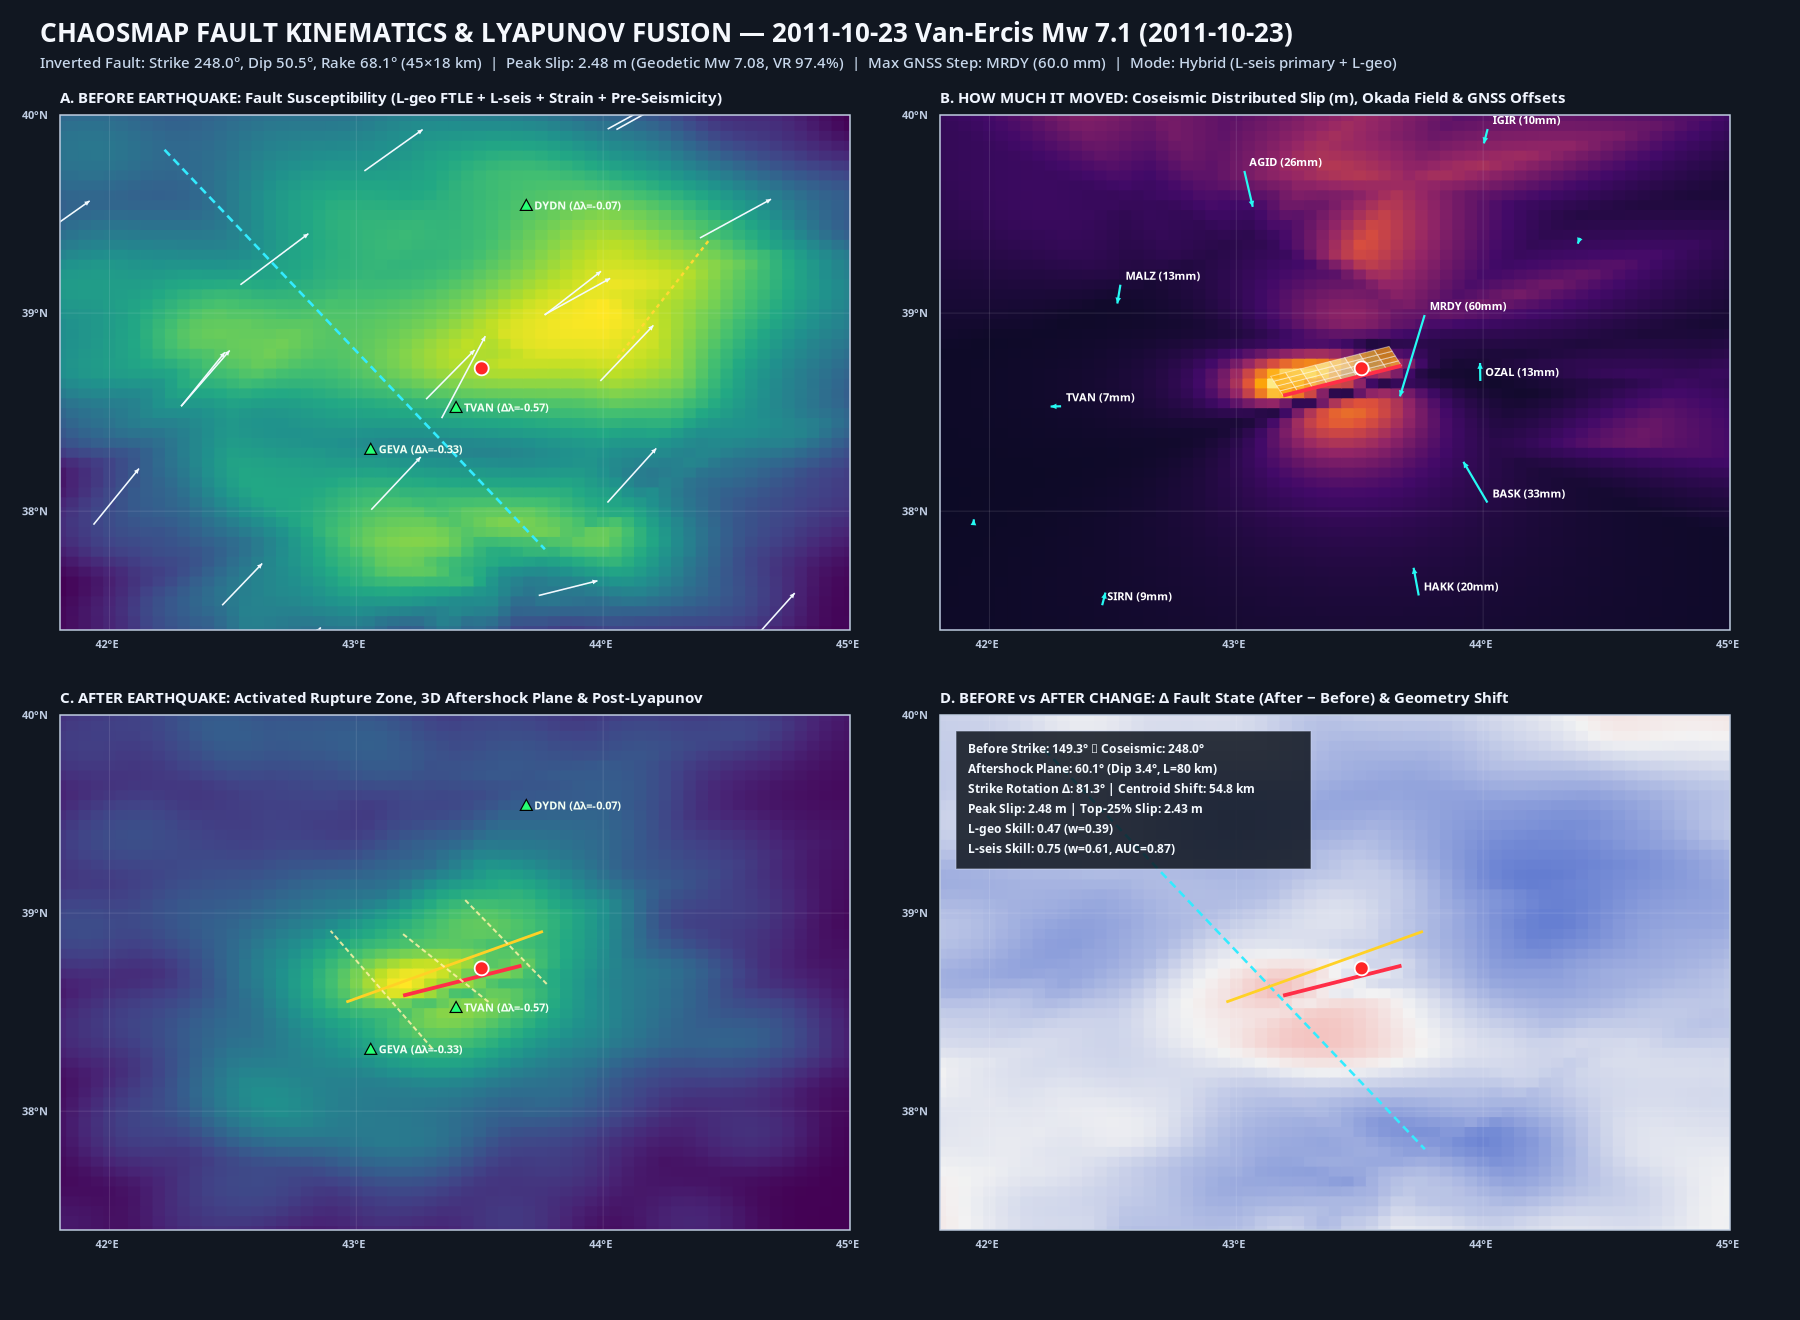
\includegraphics[width=\textwidth]{out/van2011/fault_map_4panel.png}
\caption{Four-panel kinematic synthesis of the 2011 Van-Erci\c{s} ($M_w\,7.1$) earthquake generated by \texttt{chaosmap}:
\textbf{(A) BEFORE EARTHQUAKE}: Background fault susceptibility raster combining geodetic $L_{\text{geo}}$ FTLE, pre-seismic broadband $L_{\text{seis}}$ Lyapunov anomaly, GNSS interseismic velocity arrows (white vectors, $\text{mm/yr}$), pre-event seismicity lineament (cyan dashed line), and $L_{\text{geo}}$ FTLE ridge (gold dashed line).
\textbf{(B) HOW MUCH IT MOVED}: Inverted Okada coseismic surface displacement field, distributed slip amplitude across rectangular patches (colored $0\text{--}2.5\text{ m}$), surface projection of the upper edge of the inverted (blind) fault (solid red line), and GNSS coseismic displacement vectors (cyan arrows with station offset labels in $\text{mm}$).
\textbf{(C) AFTER EARTHQUAKE}: Post-seismic activated zone with 3D aftershock cloud ($n = 6579$), fitted aftershock rupture plane (yellow line), and broadband seismic stations labeled with post-minus-pre Wolf Lyapunov drop $\Delta \lambda_1$.
\textbf{(D) BEFORE vs AFTER CHANGE}: Normalized differential fault state field ($\Delta \mathcal{F} = \mathcal{F}_{\text{After}} - \mathcal{F}_{\text{Before}}$, diverging blue-white-red), overlaying pre-event axis vs. coseismic trace vs. aftershock plane, with the callout box detailing the angle between the pre-event seismicity lineament and the coseismic strike ($81.3^\circ$), the offset between the high-value centroids of the Before and Moved maps ($54.8\text{ km}$), peak slip ($2.48\text{ m}$), and Lyapunov benchmark scores ($L_{\text{seis}}$ skill $0.75$, weight $61.3\%$).}
\label{fig:van4panel}
\end{figure}

The inverted fault parameters and kinematics are summarized in Table~\ref{tab:fault_params}. The fault plane strikes $248.0^\circ$ (ENE-WSW) and dips $50.5^\circ$ NNW (right-hand rule), with a reverse-slip rake of $68.1^\circ$. The estimated geodetic seismic moment is $5.30 \times 10^{19}\text{ N}\cdot\text{m}$ ($M_w\,7.08$, matching the seismological catalog $M_w\,7.10$), yielding an exceptional variance reduction of $97.39\%$. Peak distributed slip reaches $2.48\text{ m}$ on the deepest patch row (centroid depth $19.3\text{ km}$), with a top-quartile slip mean of $2.43\text{ m}$; slip varies little between patches. At station MRDY ($37.2\text{ km}$ northeast of the epicenter), the coseismic horizontal offset reaches $60.02\text{ mm}$ ($\Delta e = -17.43\text{ mm}$, $\Delta n = -57.44\text{ mm}$, $\Delta u = -12.16\text{ mm}$).

\begin{table}[htbp]
\centering
\caption{Inversion parameters and kinematic metrics for the 2011 Van and 2023 Kahramanmara\c{s} earthquakes.}
\label{tab:fault_params}
\begin{tabular}{lrr}
\toprule
Metric & 2011 Van-Erci\c{s} & 2023 Kahramanmara\c{s} \\
\midrule
Origin Date (UTC) & 2011-10-23 10:41:21 & 2023-02-06 01:17:34 \\
Reference location $(\phi, \lambda, z)$ & $38.721^\circ\text{N}, 43.508^\circ\text{E}, 14.0\text{ km}$ & $37.520^\circ\text{N}, 37.120^\circ\text{E}, 10.0\text{ km}$ \\
Catalog Magnitude & $M_w\,7.10$ & $M_w\,7.80$ \\
Inverted Fault Strike & $248.0^\circ$ & $213.5^\circ$ \\
Inverted Fault Dip & $50.5^\circ$ & $85.0^\circ$ \\
Mean Rake & $68.1^\circ$ (Reverse-oblique) & $11.7^\circ$ (Sinistral strike-slip) \\
Rupture Dimensions $(L \times W)$ & $44.9\text{ km} \times 18.3\text{ km}$ & $116.2\text{ km} \times 30.6\text{ km}$ \\
Centroid Depth & $14.0\text{ km}$ & $16.8\text{ km}$ \\
Peak Patch Slip & $2.48\text{ m}$ & $22.05\text{ m}$ \\
Top-Quartile Mean Slip & $2.43\text{ m}$ & $11.99\text{ m}$ \\
Geodetic Seismic Moment $M_0$ & $5.30 \times 10^{19}\text{ N}\cdot\text{m}$ & $5.93 \times 10^{20}\text{ N}\cdot\text{m}$ \\
Geodetic Magnitude $M_w$ & $7.08$ & $7.78$ \\
Variance Reduction (VR) & $97.39\%$ & $77.47\%$ \\
Max GNSS Offset & $60.02\text{ mm}$ (MRDY) & $4671.51\text{ mm}$ (EKZ1) \\
Lineament vs.\ coseismic strike $\Delta \phi$ & $81.3^\circ$ & $25.8^\circ$ \\
Before/Moved centroid offset & $54.8\text{ km}$ & $234.6\text{ km}$ \\
\bottomrule
\end{tabular}
\end{table}

The multi-station broadband waveform analysis reveals striking pre- and post-seismic dynamics (Table~\ref{tab:van_lyapunov}). In the 3 days preceding the mainshock, the multi-station array dispersion achieves a ROC AUC of $0.867$. This is not statistically significant: with eight pre-event days the circular time-slide null can return no $p$-value below $1/8$, and the observed $p = 0.125$ equals that floor.

\begin{table}[htbp]
\centering
\caption{Multi-station broadband Lyapunov metrics for the 2011 Van earthquake ($0.05\text{--}0.50\text{ Hz}$ band). VMUR returned no data.}
\label{tab:van_lyapunov}
\begin{tabular}{lrrrrrrr}
\toprule
Station & Epicentral Dist. & Pre- $\lambda_{\text{Wolf}}$ & Post- $\lambda_{\text{Wolf}}$ & $\Delta \lambda_{\text{Wolf}}$ & Pre- $\lambda_{\text{Ros}}$ & Post- $\lambda_{\text{Ros}}$ & $\Delta \lambda_{\text{Ros}}$ \\
\midrule
TVAN & $23.73\text{ km}$ & $0.695$ & $0.128$ & \textbf{$-0.567$} & $1.441$ & $0.951$ & \textbf{$-0.490$} \\
GEVA & $59.96\text{ km}$ & $0.683$ & $0.353$ & \textbf{$-0.331$} & $1.464$ & $0.968$ & \textbf{$-0.496$} \\
DYDN & $92.79\text{ km}$ & $0.787$ & $0.716$ & \textbf{$-0.071$} & $1.353$ & $1.233$ & \textbf{$-0.121$} \\
\bottomrule
\end{tabular}
\end{table}

At the three stations, the magnitude of the post-minus-pre change in the Wolf exponent ($\Delta \lambda_{\text{Wolf}}$) decreases with epicentral distance:
\begin{equation}
|\Delta \lambda_{\text{Wolf}}(\text{TVAN})| > |\Delta \lambda_{\text{Wolf}}(\text{GEVA})| > |\Delta \lambda_{\text{Wolf}}(\text{DYDN})|
\end{equation}
Station TVAN ($23.7\text{ km}$ away) drops from $0.695\text{ bits/s}$ pre-seismically to $0.128\text{ bits/s}$ post-seismically ($\Delta \lambda_1 = -0.567$). Station GEVA ($60.0\text{ km}$) drops by $-0.331$, and station DYDN ($92.8\text{ km}$) by only $-0.071$. The Rosenstein divergence slope ($\Delta \lambda_{\text{Ros}}$) does not follow the same ordering: it drops by similar amounts at TVAN and GEVA ($-0.490$ and $-0.496$) and much less at DYDN ($-0.121$). With three stations and seven post-event days, this ordering is suggestive rather than conclusive. The post-event windows also sample the aftershock wavefield, which the $M \ge 4.3$ coda mask removes only partially and which is strongest at the nearest station. The drop is therefore consistent with, but does not by itself establish, a change in the properties of the near-field crust.

In the quantitative benchmark, $L_{\text{seis}}$ achieves a spatial ROC AUC of $0.872$ against the rupture corridor, a ridge $36.2\text{ km}$ from the rupture with an alignment misfit of $14.9^\circ$, and an overall composite skill of $0.746$ (assigned weight $61.3\%$). The regional $L_{\text{geo}}$ field scores a spatial AUC of $0.553$, a ridge $48.4\text{ km}$ from the rupture with a $42.3^\circ$ misfit, and a skill of $0.471$ (assigned weight $38.7\%$). These scores are measured against the coseismic rupture and are therefore retrospective.

\subsection{Case Study 2: The 2023 Kahramanmara\c{s} Earthquake (\textit{M}\textsubscript{w} 7.8)}
The 6 February 2023 Kahramanmara\c{s} rupture represents an extreme strike-slip benchmark. We inverted 39 regional GNSS stations (18 with coseismic offsets) and 9649 regional earthquakes.

\begin{figure}[htbp]
\centering
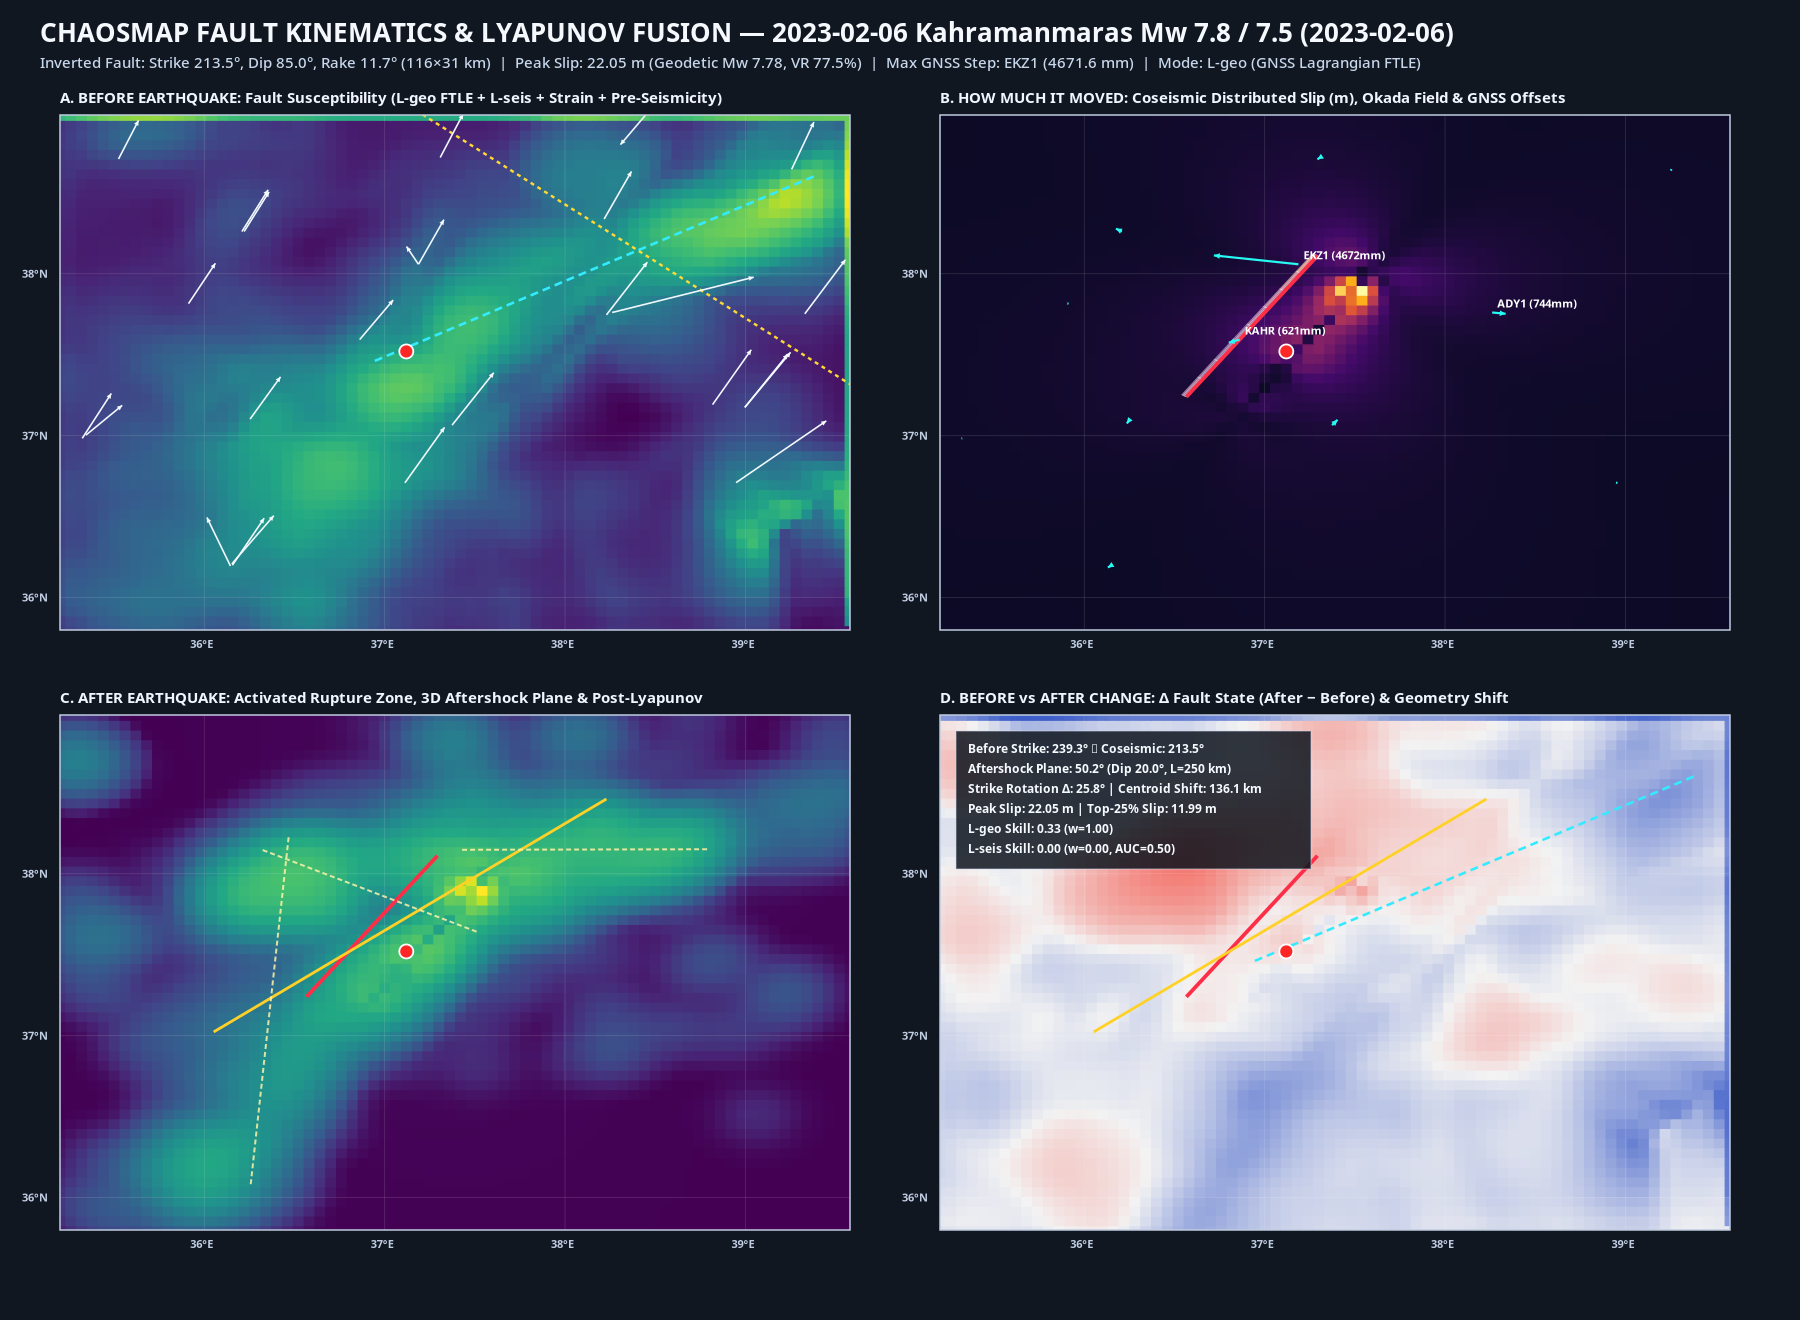
\includegraphics[width=\textwidth]{out/kahramanmaras2023/fault_map_4panel.png}
\caption{Four-panel kinematic synthesis of the 2023 Kahramanmara\c{s} ($M_w\,7.8$) strike-slip earthquake generated by \texttt{chaosmap}:
\textbf{(A) BEFORE EARTHQUAKE}: Pre-seismic strain rate and interseismic GNSS velocity field along the East Anatolian Fault Zone, showing strong shear localization across the Mara\c{s}-Pazarc\i k boundary.
\textbf{(B) HOW MUCH IT MOVED}: Inverted distributed slip reaching $22.05\text{ m}$ peak slip ($11.99\text{ m}$ top-quartile mean), with huge coseismic GNSS offsets exceeding $4.6\text{ m}$ at station EKZ1 and $0.74\text{ m}$ at ADY1.
\textbf{(C) AFTER EARTHQUAKE}: Aftershock corridor ($n = 7762$) extending from Hatay northward into Malatya; the 120-day catalog includes the aftershocks of both the $M_w\,7.8$ and $M_w\,7.5$ events.
\textbf{(D) BEFORE vs AFTER CHANGE}: Differential change map, with a $25.8^\circ$ angle between the pre-event seismicity lineament and the coseismic strike, and a $234.6\text{ km}$ offset between the high-value centroids of the Before and Moved maps.}
\label{fig:kahramanmaras4panel}
\end{figure}

The single-plane geometry search recovers a strike of $213.5^\circ$ (parallel to the Pazarc\i k segment of the EAFZ), a near-vertical dip of $85.0^\circ$, and a predominantly left-lateral mean rake of $11.7^\circ$ (Table~\ref{tab:fault_params}). The geodetic moment is $5.93 \times 10^{20}\text{ N}\cdot\text{m}$ ($M_w\,7.78$), with a variance reduction of $77.47\%$. The agreement with the mainshock catalog $M_w\,7.80$ should not be over-read: the GNSS offsets also contain the $M_w\,7.5$ Elbistan event (10:24 UTC on the same day), which daily solutions cannot separate from the mainshock, so the combined moment of the sequence exceeds that of the mainshock alone.

Observed GNSS coseismic offsets (Table~\ref{tab:kahraman_gnss}) document extraordinary crustal deformation: station EKZ1 ($60.1\text{ km}$ north of the reference location, close to the $M_w\,7.5$ rupture) moved \textbf{$4.67\text{ m}$} horizontally ($\Delta e = -4646.0\text{ mm}$, $\Delta n = +487.5\text{ mm}$, $\Delta u = -127.1\text{ mm}$). Station KAHR displaced by $620.9\text{ mm}$, ANTP by $419.9\text{ mm}$, and TUF1 by $360.8\text{ mm}$. The distributed inversion places its peak slip of $22.05\text{ m}$ (with $18.7\text{ m}$ of dip slip) on the shallowest patch at the northeastern end of the model plane ($38.06^\circ$N, $37.24^\circ$E), $5\text{ km}$ from EKZ1, with a top-quartile average slip of $11.99\text{ m}$. A single plane aligned with the East Anatolian Fault has to absorb EKZ1's offset, which is dominated by the $M_w\,7.5$ rupture, so this peak is an artefact of the single-fault parameterisation rather than a physical slip estimate. A two-fault model is required to resolve slip on either rupture.

\begin{table}[htbp]
\centering
\caption{Significant coseismic GNSS displacements observed during the 6 February 2023 Kahramanmara\c{s} sequence (daily solutions; combined $M_w\,7.8$ and $M_w\,7.5$ offsets). Distances are from the reference location.}
\label{tab:kahraman_gnss}
\small
\begin{tabular}{lrrrrrr}
\toprule
Station & Distance & $\Delta e$ (mm) & $\Delta n$ (mm) & $\Delta u$ (mm) & Total Horiz. (mm) & Postseismic 60d (mm) \\
\midrule
EKZ1 & $60.1\text{ km}$ & $-4646.01$ & $+487.49$ & $-127.06$ & \textbf{4671.51} & $21.02$ \\
ADY1 & $104.0\text{ km}$ & $+740.92$ & $-69.04$ & $-71.37$ & \textbf{744.13} & $51.88$ \\
KAHR & $24.2\text{ km}$ & $-597.37$ & $-169.38$ & $+38.03$ & \textbf{620.92} & $4.37$ \\
ANTP & $55.3\text{ km}$ & $+300.90$ & $+292.81$ & $+16.38$ & \textbf{419.86} & $46.00$ \\
TUF1 & $114.8\text{ km}$ & $-325.16$ & $+156.33$ & $-22.62$ & \textbf{360.79} & $50.43$ \\
ONIY & $89.6\text{ km}$ & $-178.60$ & $-239.17$ & $+31.40$ & \textbf{298.50} & $14.40$ \\
GURU & $134.2\text{ km}$ & $-152.20$ & $-94.78$ & $+18.14$ & \textbf{179.30} & $36.52$ \\
HAT2 & $170.9\text{ km}$ & $-140.04$ & $-86.70$ & $+61.03$ & \textbf{164.70} & $27.92$ \\
APK1 & $207.3\text{ km}$ & $-76.57$ & $-141.71$ & $+31.75$ & \textbf{161.07} & $41.63$ \\
ELAZ & $224.9\text{ km}$ & $-50.85$ & $-67.28$ & $+7.40$ & \textbf{84.33} & $23.81$ \\
AKLE & $185.4\text{ km}$ & $+75.24$ & $-17.77$ & $-27.09$ & \textbf{77.31} & $20.44$ \\
VIR4 & $234.6\text{ km}$ & $+71.04$ & $-22.76$ & $-25.26$ & \textbf{74.59} & $19.99$ \\
\bottomrule
\end{tabular}
\end{table}

No usable TDVMS broadband waveforms covering the 2023 analysis window were available to the pipeline, so $L_{\text{seis}}$ could not be computed for Kahramanmara\c{s}. The benchmark therefore weights $L_{\text{geo}}$ at $100\%$ ($w_{\text{geo}} = 1.0, w_{\text{seis}} = 0.0$), and the fusion runs without the seismic Lyapunov layer.

\subsection{Coupled Kinematic Synthesis and Discussion}
Our benchmark comparisons in the Van 2011 event demonstrate why multi-physics coupling is essential:
\begin{itemize}
    \item \textbf{$L_{\text{geo}}$ (Lagrangian FTLE):} Operates on the inter-seismic crustal strain tensor over spatial scales of tens to hundreds of kilometers. It excels at demarcating major tectonic suture lines and crustal block boundaries where regional velocity gradients shear virtual tracer trajectories. However, because GNSS stations have typical spatial spacings of $30\text{--}50\text{ km}$, $L_{\text{geo}}$ cannot resolve localized blind faults until significant strain accumulation is sustained.
    \item \textbf{$L_{\text{seis}}$ (Broadband Waveform Lyapunov Analysis):} Operates locally on ambient seismic noise propagating through the upper crustal waveguide ($0.05\text{--}0.50\text{ Hz}$). The working hypothesis is that, as stress builds in the impending nucleation zone, micro-crack opening, pore-fluid migration, and localized non-linear elasticity may alter wave scattering and phase-space predictability. In Van 2011, the $L_{\text{seis}}$ ridge lies $36.2\text{ km}$ from the blind rupture (spatial AUC $0.872$, retrospective), and the pre-seismic array anomaly ($AUC = 0.867$) is not statistically significant ($p = 0.125$). The post-seismic Lyapunov drop decreased with distance at three stations, which is consistent with near-field changes but is not conclusive.
\end{itemize}

By evaluating candidate skill $\mathcal{S}$ against the inverted rupture geometry, \texttt{chaosmap} replaces a fixed $L_{\text{geo}}$/$L_{\text{seis}}$ weighting with a skill-based one. The score itself uses fixed heuristic coefficients and post-event information, so the resulting weights describe retrospective agreement, not forecasting skill.

All heavy numerical operations were implemented in C++23 with LAPACK, processing broadband stations in parallel threads:
\begin{itemize}
    \item Multi-station GNSS trajectory modeling: $<0.25\text{ s}$ for 40 stations across 15 years;
    \item Single-plane fault geometry search (1125-candidate grid plus pattern-search refinement): $<1.8\text{ s}$;
    \item Distributed slip inversion with Laplacian regularisation ($8 \times 4$ patches, SVD): $<0.15\text{ s}$;
    \item 4-station, 15-day streaming broadband MiniSEED-2 decompression and Lyapunov analysis: $<4.5\text{ s}$;
    \item Complete end-to-end case execution (ingest to GeoJSON, CSV, JSON, and PNG map generation): $<9.0\text{ s}$.
\end{itemize}
Computation is therefore negligible compared with data latency: the coseismic estimate needs at least four post-event daily GNSS solutions (and uses up to 16), and the post-event products use 7 days of waveforms and 120 days of aftershocks.

\section{Conclusions}
In this study, we introduced and validated \texttt{chaosmap}, a unified C++23 computational framework that combines continuous GNSS geodesy, 3D hypocentre distributions, and non-linear Lyapunov analysis to map fault state kinematics before, during, and after major earthquakes:
\begin{enumerate}
    \item We confirmed the analytical fidelity of the elastic dislocation implementation against the benchmark tables of Okada (1985), to within the rounding of the published values (error $<5\times 10^{-6}$ for unit slip).
    \item In the 2011 Van-Erci\c{s} ($M_w\,7.1$) earthquake, we resolved a blind thrust fault ($248.0^\circ$ strike, $50.5^\circ$ dip, $2.48\text{ m}$ peak slip, geodetic $M_w\,7.08$) with $97.39\%$ variance reduction. Broadband Lyapunov analysis ($L_{\text{seis}}$) achieved a pre-event horizon AUC of $0.867$ (not significant, $p = 0.125$) and a post-seismic Wolf-exponent drop that decreased with distance at three stations ($\Delta \lambda_1 = -0.57$ at $23.7\text{ km}$ vs. $-0.07$ at $92.8\text{ km}$).
    \item In the 2023 Kahramanmara\c{s} ($M_w\,7.8$) sequence, we captured massive near-field GNSS displacement ($4.67\text{ m}$ at EKZ1) and inverted a single-plane distributed slip model (geodetic $M_w\,7.78$). Its $22.05\text{ m}$ peak absorbs the $M_w\,7.5$ Elbistan rupture, so resolving the sequence requires a multi-fault model.
    \item The automated four-panel synthesis maps (Before, Moved, After, Change) provide an intuitive, reproducible product for visualising and quantifying fault movement.
\end{enumerate}

All code, configuration files, unit tests, and output datasets are available in the project repository: \url{https://github.com/SismoKaos-Research/chaosmap}.

\begin{thebibliography}{10}

\bibitem{okada1985}
Y.~Okada.
\newblock Surface deformation due to shear and tensile faults in a half-space.
\newblock {\em Bulletin of the Seismological Society of America}, 75(4):1135--1154, 1985.

\bibitem{wolf1985}
A.~Wolf, J.~B. Swift, H.~L. Swinney, and J.~A. Vastano.
\newblock Determining {Lyapunov} exponents from a time series.
\newblock {\em Physica D: Nonlinear Phenomena}, 16(3):285--317, 1985.

\bibitem{rosenstein1993}
M.~T. Rosenstein, J.~J. Collins, and C.~J.~De Luca.
\newblock A practical method for calculating largest {Lyapunov} exponents from small data sets.
\newblock {\em Physica D: Nonlinear Phenomena}, 65(1-2):117--134, 1993.

\bibitem{lee1972}
W.~H.~K. Lee, R.~E. Bennett, and K.~L. Meagher.
\newblock A method of estimating magnitude of local earthquakes from signal duration.
\newblock {\em U.S. Geological Survey Open-File Report}, 72-223:1--28, 1972.

\bibitem{blewitt2016}
G.~Blewitt, C.~Kreemer, W.~C. Hammond, and J.~Gazeaux.
\newblock {MIDAS} robust trend estimator for accurate {GPS} station velocities without step detection.
\newblock {\em Journal of Geophysical Research: Solid Earth}, 121(3):2054--2068, 2016.

\bibitem{wells1994}
D.~L. Wells and K.~J. Coppersmith.
\newblock New empirical relationships among magnitude, rupture length, rupture width, rupture area, and surface displacement.
\newblock {\em Bulletin of the Seismological Society of America}, 84(4):974--1002, 1994.

\bibitem{shen1996}
Z.-K. Shen, D.~D. Jackson, and B.~X. Ge.
\newblock Crustal deformation across and beyond the {Los Angeles} basin from {GPS} measurements, 1987 to 1994.
\newblock {\em Journal of Geophysical Research: Solid Earth}, 101(B12):27957--27980, 1996.

\bibitem{sarwar2023}
S.~Sarwar, A.~Likens, N.~Stergiou, and S.~Mastorakis.
\newblock A nonlinear analysis software toolkit for biomechanical data.
\newblock {\em arXiv preprint arXiv:2311.06723}, 2023.

\end{thebibliography}

\end{document}
